% Week 3: limitations of BAKMM-IoD, related work, research gap, FSL-AKE-IoD (v2), architecture,
% security and performance analysis.  Needs: booktabs, graphicx, amsmath, amssymb, longtable.
% Every number in this file is produced by proposed/code/*.py (see VERIFICATION_LOG.md).

\subsection{Limitations of BAKMM-IoD (verified)}
\label{subsec:w3-limitations}

All checks were run on a re-implementation of the drone ($DE_i$) to ground station ($ES_j$) phase
(\texttt{bakmm\_iod.py}) and on a literal transcription of the printed equations (\texttt{bakmm\_literal.py}).
The adversary is the paper's own: Dolev--Yao, CK, and physical drone capture with power analysis (\S3.2 of~[1]).
Table~\ref{tab:w3-flaws} summarises the verdicts.

\begin{table}[ht]
\centering
\caption{Claimed BAKMM-IoD flaws after independent verification.}
\label{tab:w3-flaws}
\small
\begin{tabular}{p{0.9cm}p{4.6cm}p{2.3cm}p{6.2cm}}
\toprule
Id & Flaw & Verdict & Evidence / condition \\
\midrule
A0 & Printed SK concatenation order differs between ES (AKDDE2) and DE (AKDDE3, Table 5) & CONFIRMED (erratum) & 0/1000 sessions agree with the printed formulas \\
A1 & Drone capture reveals all past and future SKs and links the TID chain & CONFIRMED & 5/5 past, 3/3 future SKs; contradicts Prop.~5, ASFF8, ASFF13, \S3.2 (forward secrecy). Not ASFF10. \\
A2 & Stolen ES table lets the adversary impersonate every drone; $TC_{DE}$ never checked & CONDITIONAL & needs read access to the ES database, which Prop.~4 assumes is prevented; the $TC_{DE}$ part is unconditional \\
A3 & One dropped message locks the drone out & CONFIRMED & both readings of the ES update (drop MSG3 / drop MSG2) \\
A4 & Replay of MSG1 inside $\Delta T$ & CONFIRMED / CONDITIONAL & accepted if the ES commits on MSG3; lock-out needs a single pending slot; rejected if the ES commits on MSG2 \\
A5 & \textbf{New:} M5 is not covered by M4; one flipped bit locks the drone out & CONFIRMED & both policies; contradicts Prop.~2 and ASFF2 \\
E & ES--CS phase as printed does not run & CONFIRMED & m1/m2 inner-hash order differ (CS m2 check fails); ES recovers $TIN^{new}$ with $RS_2$ it never learns \\
C & \S7.2 arithmetic & CONFIRMED & $704+800+288=1792$; the printed ``2880'' and ``1782'' are typos \\
\bottomrule
\end{tabular}
\end{table}

\paragraph{Why A1 is not caught by the paper's Scyther model.}
The paper's SPDL (Fig.~3/4) declares \texttt{const xor: Function}, an uninterpreted symbol without the cancellation
law. In such a model the intruder can never remove a mask $V\oplus h(RID_{DE}\|MS\|T)$, whatever it knows.
The ``no attacks within bounds'' result therefore says nothing about capture resistance.
The repository contains a capture model that encodes masking as encryption keyed by the mask
(\texttt{bakmm\_auth\_compromise.spdl}); its expected result is a failed SK secrecy claim.

\subsection{Comparison with related schemes}
\label{subsec:w3-related}

Security attributes are taken from Table~10 of~[1] (ASFF identifiers) unless marked ``unresolved''.
The source papers of~[2]--[4] are not in the repository, so the attributes that Table~10 does not cover
(forward secrecy, stolen verifier, de-synchronisation) could not be verified and are left as ``unresolved''.

\begin{table}[ht]
\centering
\caption{BAKMM-IoD, three related schemes and FSL-AKE-IoD (v2). Costs from Tables~8--9 of~[1]; ``*'' = broken in this work.}
\label{tab:w3-related}
\small
\begin{tabular}{p{3.0cm}p{2.1cm}p{2.1cm}p{2.1cm}p{2.1cm}p{2.3cm}}
\toprule
 & Bera et al.~[2] & Mishra et al.~[3] & Algarni \& Jan~[4] & BAKMM-IoD~[1] & FSL-AKE-IoD v2 \\
\midrule
Primitives & hash, ECC, AES & hash & hash (MD5), fuzzy extr. & hash, XOR & hash \\
Drone cost & $9T_h{+}2T_{senc}{+}2T_{ecm}{+}T_{eca}$ 7.405\,ms & $9T_h$ 2.78\,ms & $T_{fe}{+}14T_h$ 6.614\,ms & $8T_h$ 2.47\,ms & $5T_h$ 1.545\,ms \\
Server cost & 1.851\,ms & $7T_h$ 0.39\,ms & $6T_h$ \textbf{0.33\,ms} & $8T_h$ 0.44\,ms & $7T_h$ 0.385\,ms \\
Messages / bits & 3 / 2368 & 3 / 1792 & 4 / 2784 & 3 / 1792 & \textbf{2 / 1056} \\
Replay (ASFF1) & yes & yes & yes & no* (in $\Delta T$) & yes (cache to $T_1{+}\Delta T$) \\
Capture (ASFF8) & yes & yes & yes & no* & past: yes; KCI/future: no \\
Forward secrecy & unresolved & unresolved & unresolved & no* & drone side yes \\
Stolen verifier & unresolved & unresolved & unresolved & no* (if DB read) & yes (needs SE for $X_{ES}$) \\
De-sync resilience & unresolved & unresolved & unresolved & no* & yes (F3, F4) \\
Anonymity (ASFF13) & yes & yes & no & no* (after capture) & partial (retries linkable) \\
ESL (ASFF10) & yes & yes & no & yes & yes (vacuous: nonces public) \\
Dynamic addition (ASFF11) & yes & yes & no & yes & yes \\
Blockchain (ASFF12) & yes & no in~[1] Table~10 & no & yes & yes \\
Formal verification (ASFF9) & yes & yes & yes & $\times$ in Table~10 (Scyther in \S6) & models written, not run \\
\bottomrule
\end{tabular}
\end{table}

\subsection{Research gap}
\label{subsec:w3-gap}

\begin{enumerate}
\item \textbf{Forward secrecy at hash-only cost.} The hash-only IoD schemes derive every session key from static long-term
secrets (for BAKMM-IoD, verified: A1). ECC-based schemes can obtain forward secrecy but cost about $3\times$ more on the drone.
\item \textbf{Capture is argued, not modelled.} The published Scyther models omit key reveal and treat XOR as an uninterpreted function,
so capture attacks are invisible to them.
\item \textbf{State synchronisation.} Pseudonym rotation without a recovery path turns one lost or modified message into a permanent
lock-out (A3, A5).
\item \textbf{Edge verifier tables.} Ground stations are field-deployed yet store per-drone master keys in the clear (A2).
\item \textbf{Cost.} Among the compared schemes, FSL-AKE-IoD v2 is the cheapest on the drone and in communication,
but not on the server (Algarni \& Jan: $6T_h$).
\end{enumerate}

\subsection{Proposed protocol: FSL-AKE-IoD (v2)}
\label{subsec:w3-protocol}

$DE_i$ stores $\{TID_i,K_i\}$. $ES_j$ keeps $X_{ES}$ in a secure element and stores masked records
$C_i=K_i\oplus h(X_{ES}\|TID_i)$.
\begin{align}
MSG_1 &= \{TID,N_1,T_1,V_1\}, & V_1 &= h(K\|TID\|N_1\|T_1) & (608~\text{bits})\\
SK &= h(K\|N_1\|N_2\|T_1\|T_2\|TID), & & & \\
MSG_2 &= \{N_2,T_2,V_2\}, & V_2 &= h(SK\|N_2\|T_2) & (448~\text{bits})\\
K &\leftarrow h(K\|SK), & TID &\leftarrow h(TID\|SK)_{[0..159]} &
\end{align}
The review of the draft version (v1) found four flaws and fixed them:
\textbf{F1}, a unique device id per drone (v1's default id made one drone's session delete every other drone);
\textbf{F2}, replay-cache entries kept until $T_1+\Delta T$ rather than receive time $+\Delta T$ (otherwise a replay
under legal clock skew is accepted and locks the drone out);
\textbf{F3}, the ES keeps the last proven key as the \emph{anchor} plus every \emph{candidate} derived from it, and
promotes a candidate only when the drone proves it holds it (v1's single old/current pair is broken by a reordered
retry);
\textbf{F4}, the drone waits more than $2\Delta T$ before re-sending on the same credentials, so the bounded candidate
list cannot be evicted.
In addition, the ES refuses $MSG_1$ for $2\Delta T$ after a reboot, tries every record stored under a TID
(collision tolerance), and revocation deletes the anchor and all candidates. The ES--CS key management uses the same
exchange with $ES_j$ as initiator.

\subsection{Architecture}
\label{subsec:w3-arch}

The architecture has four layers: drones (5 hash operations per session); ground stations (secure element, masked
anchor and candidate records, replay cache, ECC/ECDSA partial blocks); cloud servers (P2P, pBFT); and the offline RA,
which must erase $K_i$ after provisioning. Figure sources are \texttt{fslake\_architecture.dot} and
\texttt{fslake\_auth.dot}; the SVGs are in the repository root.

\subsection{Security analysis}
\label{subsec:w3-security}

32 attacks were run against BAKMM-IoD (both ES update policies), the draft protocol (v1) and v2
(\texttt{attacks\_fslake.py}, reproduced by \texttt{tests/test\_protocols.py}). Nine attacks succeed against v1:
replay under clock skew, replay after an ES reboot, a reordered retry, withheld-retry eviction, a second drone's
record being deleted, naive revocation, TID-collision overwrite, and the two inherent ones below. v2 resists all of
these. The limitations that remain for v2 are inherent to a symmetric-key-only design, or are partial:
\begin{itemize}
\item KCI after drone capture, and future sessions after capture (no post-compromise security);
\item full ES compromise with $X_{ES}$ exposes the last session of each drone (3/15 in the experiment) and all future ones;
      adding a key-confirmation $MSG_3$ lowers this to 0/15 without ECDH;
\item failed attempts reuse the TID, so an active adversary that drops MSG2 can track a drone (optional retry pseudonyms remove this at $+w$ ES hashes);
\item an RA that keeps $K_0$ and records every transcript learns every SK (the chain breaks after one missed transcript);
\item clock drift beyond $\Delta T$ and roaming across ground stations with one credential.
\end{itemize}
The ablation (\texttt{ablation.py}) shows that each of M1--M5 and F2--F4 is necessary: switching one off re-opens a
specific attack. M6 (two messages) re-opens nothing; it is a cost optimisation that gives up ES-side forward secrecy
of the last session.
A Real-or-Random proof sketch is in \texttt{FSL-AKE-IoD-security\_verification.ipynb}; its bound is
$\mathrm{Adv}\le q_h^2/2^{256}+(q_s+q_e)^2/2^{160}+(2q_s+2q_h)/2^{256}$.
Scyther and ProVerif models (plain, capture, and a control model) were written but \textbf{not run}, because
neither tool is installed on the authoring machine.

\subsection{Performance analysis}
\label{subsec:w3-performance}

Hash counts were obtained by instrumenting $h(\cdot)$: BAKMM-IoD takes 8 on the drone (3+5) and 8 on the ES (7+1);
FSL-AKE-IoD v1 and v2 both take 5 and 7. With the paper's $T_h$ (0.309\,ms Raspberry Pi~3, 0.055\,ms server), the drone
cost falls from 2.472 to 1.545\,ms ($-37.5\%$), the server cost from 0.440 to 0.385\,ms ($-12.5\%$), and
communication from 1792 to 1056 bits ($-41.1\%$, 3$\to$2 messages).
FSL-AKE-IoD v2 has the lowest drone cost and the lowest communication of all compared schemes. On the server it is
\textbf{not} the cheapest: Algarni \& Jan need $6T_h$ (0.33\,ms), and Mishra et al.\ equal it at $7T_h$.
On the authoring PC one SHA-256 call through $h(\cdot)$ took about $7\,\mu$s on average ($10^5$ runs), and a full
FSL-AKE-IoD session took less time than a BAKMM-IoD session.

\begin{figure}[ht]
\centering
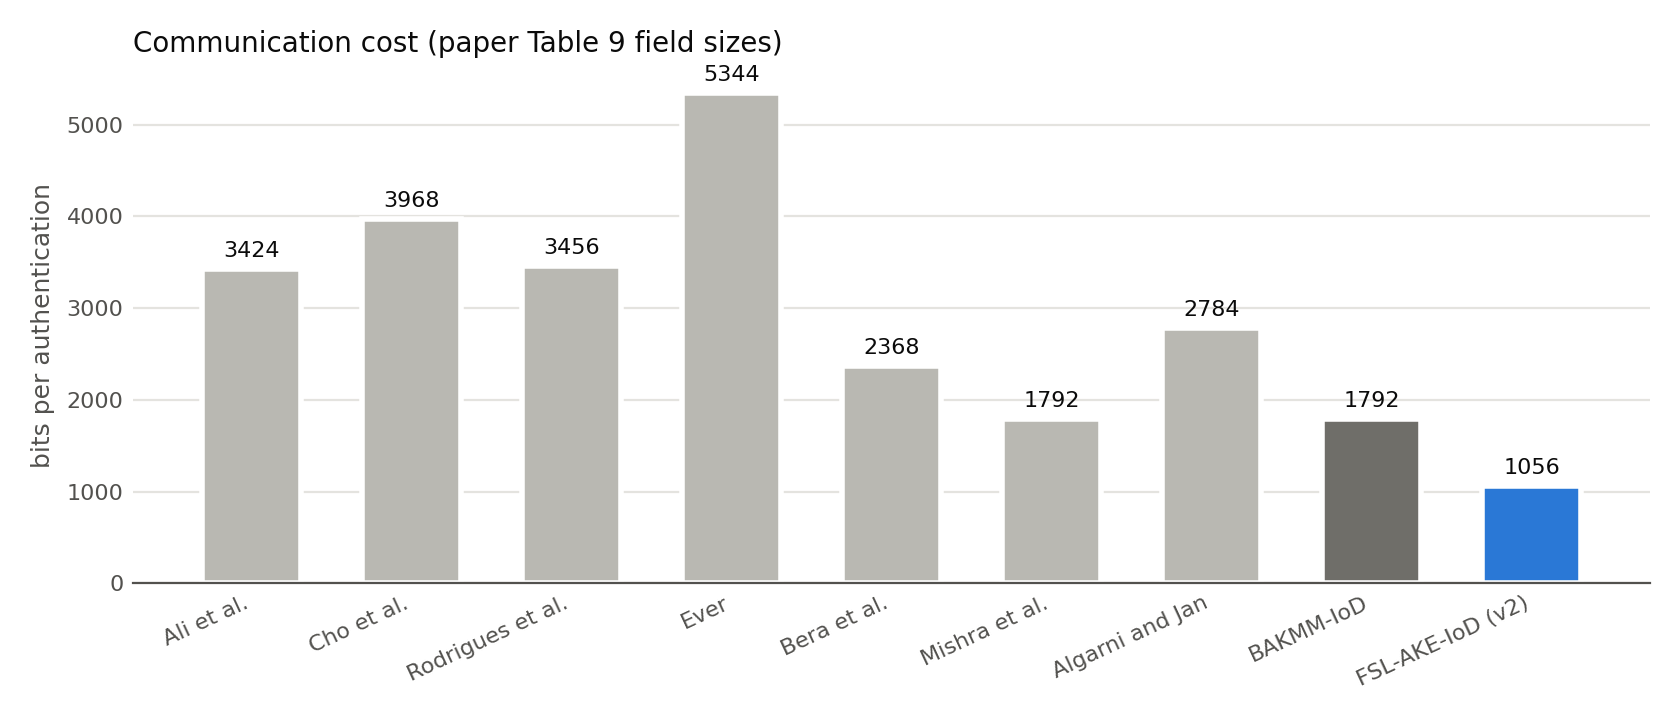
\includegraphics[width=0.48\textwidth]{images/fslake_comm_cost.png}\hfill
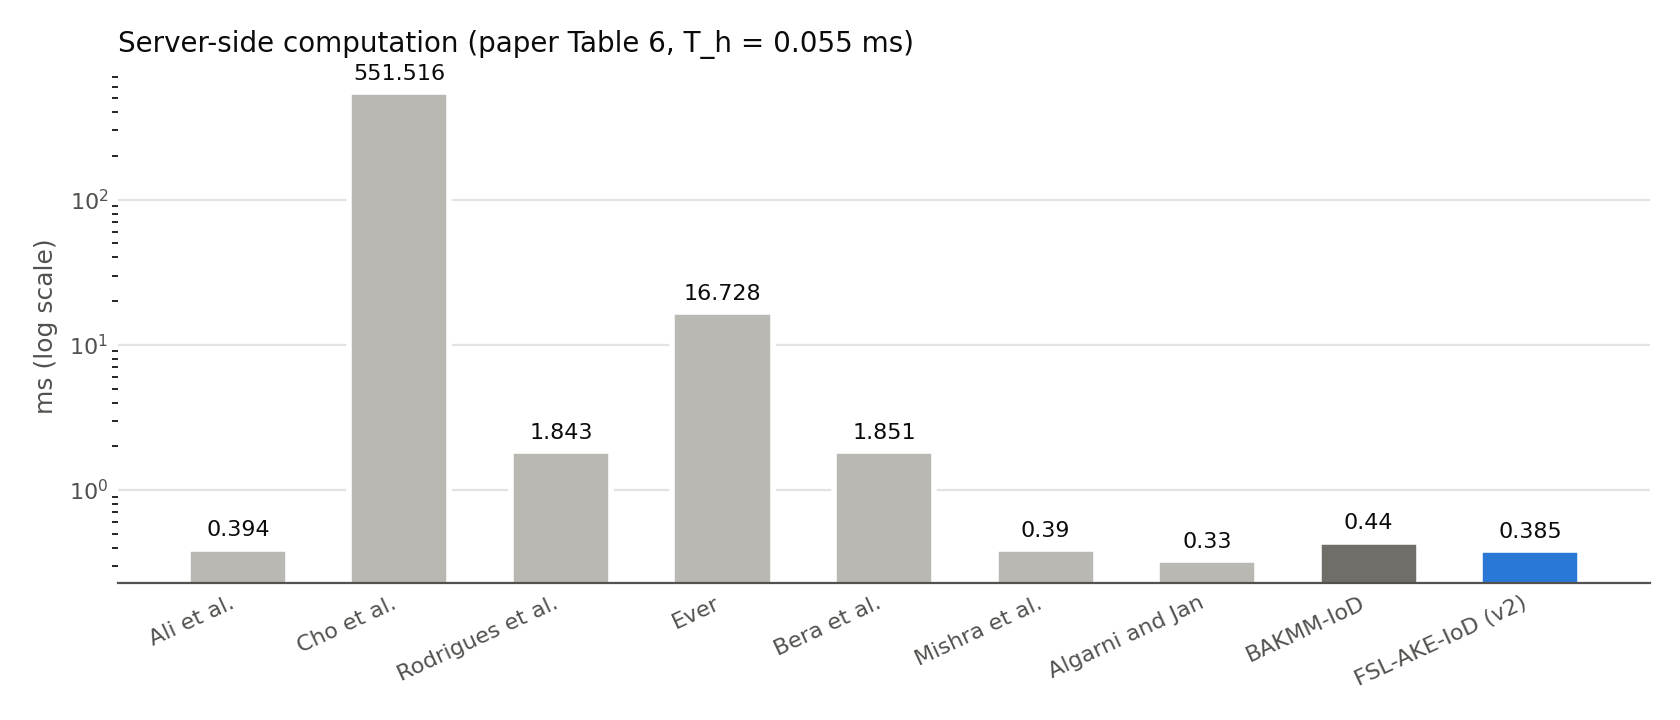
\includegraphics[width=0.48\textwidth]{images/fslake_server_cost.png}
\caption{Communication cost and server-side computation (Tables~8--9 of~[1] plus FSL-AKE-IoD v2).}
\label{fig:w3-cost}
\end{figure}
